% !TEX root = ../thesis.tex
%
\chapter{Related Work}
\label{sec:related}

As Runtime Monitoring and Verification is a widely researched field, multiple approaches to attain it's goals were developed.

As stated in~\cite{Havelund2008} most approaches are geared towards software written in Java, while many critical systems are written in C and there are countless other systems that could benefit from monitoring and verification written in all kinds of programming languages.
With \gls{tessla} as a specification language over streams, which has no assumptions on the environment of the system that produces the streams,  as the base for our monitoring approach, we recognized the possibility to abstract the monitoring platform from the monitored program.
This means that the developed runtime for \gls{tessla} is not restricted to monitor programs written in a specific language but can monitor anything that can produce streams of data.

To show that the runtime is valuable in the context of existing approaches, we will show ways to generate traces from systems that were used to evaluate other monitoring techniques.
Based on the generated traces the runtime will be benchmarked to see how it scales with respect to different characteristics of specifications and the plattform it is run on.

The following chapter will summarize the approaches that are available in the field of \gls{rv} and how they influence \gls{tessla} and the implemented runtime.

\section{\glsentryname{rv} Techniques for C Programs}
\label{sec:related:c_programs}
\subsection{Copilot}
\label{sec:related:c_programs:copilot}

The realtime runtime monitor system Copilot was introduced in~\cite{Pike2010}.
Copilot is designed to overcome the shortcomings of existing \gls{rv} tools in regards to hard-realtime software written in C.

To do so they first define characteristics a monitoring approach has to fullfill to be considered valuable for this domain.
The four principles are:

\begin{description}
  \item[Functionality] Monitors cannot change the functionality of the observed program unless a failure is observed.
  \item[Schedulability] Monitors cannot alter the schedule of the observed program.
  \item[Certifiability] Monitors must minimize the difficulty in re-validating the observed program; in particular, we make it our goal to avoid modifying the observed programs source code.
  \item[SWaP overhead] Monitors must minimize the additional overhead required including size, weight, and power (SWaP).
\end{description}

The monitors follow a sampling based approach, where at specified steps the values of global variables are observed and the monitors are evaluated
on that values.
While sampling based approaches are widely disregarded in \gls{rv}, because they can lead to both false positives and false negatives,
they argue:

\begin{quote}
  In a hard real-time context, sampling is a suitable strategy.
  Under the assumption that the monitor and the observed program share a global clock and a static periodic schedule, while false positives are possible, false negatives are not.~\cite{Pike2010}
\end{quote}

A special detail of Copilot is that monitors aren't inlined into the program but can be scheduled as independet processes.
The implementation of the \gls{tessla} runtime in this thesis follows a similar approach: It is a totally independent program,
and therefore also has some of the gains in regard to the specified four characteristics.
Because the runtime works with all kinds of traces, it is insignificant how they are produced:
It can work with traces based on sampling, working in a similar fashion as Copilot, or by actually instrumenting code to generate
traces, which alters the semantics of the program.

\subsection{\glsentryname{rmor}}
\label{sec:related:c_programs:rmor}

\gls{rmor}~\citep{Havelund2008} is another approach on monitoring C programs.
It does so by transforming C code into an \emph{armored} version, which includes monitors to check conformance to a specification.

Specifications are given as a textual representation of state machines, which is strongly influenced by \gls{rcat}~\citep{Smith2008}.
The specifications are then interweaved into the program using CIL~\cite{Necula2002}.
Specifications work on the level of function calls and state properties like \emph{write may never be called before open was called}.
Because software developers are often working at the same abstraction level (in contrast to e.g.\ assembler or machine instructions), they can define specifications without having to learn new concepts.
In the \gls{tessla} runtime support for traces at the same abstraction level (function calls, variable reads and writes) is present and used in most of the tests in \Cref{sec:evaluation:runtime_examples}.

Because \gls{rmor} specifications are interweaved into the program, their observations can not only be reported but also used to recover the program or even to prevent errors by calling specified functions when a critical condition is encountered.
The \gls{tessla} runtime doesn't support this out of the box, as it's primary purpose is testing and offline monitoring, but in \Cref{sec:conclusion:further_work:error_prevention} we will look at possible extensions to support this.

\section{Distributed Verification Techniques}
\label{sec:related:distributed}

Many works in the field of \gls{rv} don't consider the modern reality of parallelism and distributed system.
There are two aspects to this challenge: monitoring programs that are run in a distributed fashion on the one hand and using parallelism and distribution to implement monitors on the other.

Monitoring distributed programs carries an inherent problem: Events are no longer globally ordered.
This led to algorithms like Lamport timestamps~\citep{Lamport1978} and vector clocks~\citep{Fidge1988}.
The distribution of the monitored system, and therefore of the events, must be expressable in the language that is used to write specifications about the system.
Two examples for such a specification language are presented in \cite{Sen2004} and \cite{Ehrich2000}.
In~\cite{Mostafa2015} a way to monitor distributed programs is presented that uses \gls{ltl} as the specification language but requires the presence of a global state which is cosntructed using Lamport timestamps.
To do this distributed monitors, which have to communicate with one another, are specified and implemented.

The other challenge of parallelism and distribution is how it can be included in monitoring algorithms.
Since modern systems often contain many processor core it wouldn't be efficient to ignore this fact when building monitors, especially when performance of the monitor is important.

The work in~\cite{Attard2016} uses the Erlang plattform to implement a highly distributed monitoring algorithm.
It achieves this by synthesizing formulas into \emph{submonitors} which can then be run in parallel and their verdicts are combined to form a global verdict.
For example the formula \(\Phi \vee \Psi\) can be synthesized as two \emph{submonitors}, one for \(\Psi\) and one for \(\Phi\).

Whle the \gls{tessla} specification language doesn't include mechanisms to explicitly reason about distributed properties, the \gls{tessla} runtime doesn't care about the environment of the monitored program, so it doesn't distinguish between traces from distributed and non distributed programs.
As we will see in \Cref{sec:implementation:tesslaserver} this means that with a trick \gls{tessla} can be used to monitor at least some characteristics of a distributed system.
But more important is that the runtime takes parallelism and distribution as one of its core concepts as we will see in the next chapters.


\section{Stream Based Specification Techniques}
\label{sec:related:stream_based}
\subsection{\glsentryname{lola}}
\label{sec:related:stream_based:lola}

The concepts of \gls{lola}~\cite{DAngelo2005} are very similar to the ones of \gls{tessla}.
Both approaches built upon streams of events.
The biggest difference between them is, that while streams in \gls{lola} are based on a discrete model of time \gls{tessla} uses a continuous timing model.

The specification language of \gls{lola} is very small (expressions are built upon three operators) but the expressiveness surpasses \glspl{tl} and many other formalisms \citep{DAngelo2005}.
Expressions in \gls{lola} are built by manipulating existing streams to form new ones.
Therefore streams depend on other streams, so they can be arranged in a weighted dependency graph, where the weight describes the amount of steps a generated stream is delayed compared to the parent.
In contrast to \gls{tessla} streams in \gls{lola} can depend on themself and therefore the dependency graph can contain cycles.

Based on this graph a notion of efficiently monitorable properties is given and an algorithm to monitor them is presented.

\gls{tessla} takes concepts of \gls{lola} and applies them to a continuous model of time and introduces a language and a rich set of functions that can be applied to streams.
The dependency graph is a core concept of \gls{tessla} and is used to check if specifications are valid (e.g.\ cycle free) and is also the core concept to evaluate specifications over traces in this thesis.

\subsection{BeepBeep 3}
\label{sec:related:stream_based:beepbeep}
TODO: Sync event stream processing.
Note the concept of the front.

\section{\glsentryname{tessla}}
\label{sec:related:tessla}

The implemented runtime and the theoretic work of this thesis is built upon the \gls{tessla} project from~\cite{Decker2016}.
For that project a syntax and a formal semantic of a specification language was defined.

Specifications in \gls{tessla} are based on streams of data.
Streams are the representation of data over time, e.g.\ a variable value in a program or the temperature of a processor.
To model streams \gls{tessla} defines a timing model.
That model is based on timestamps that are isomorphic to real numbers \(\mathbb{R}\).
\Cref{fig:chap2:sec_tessla:streams} shows how streams behave over time.

\begin{figure}
  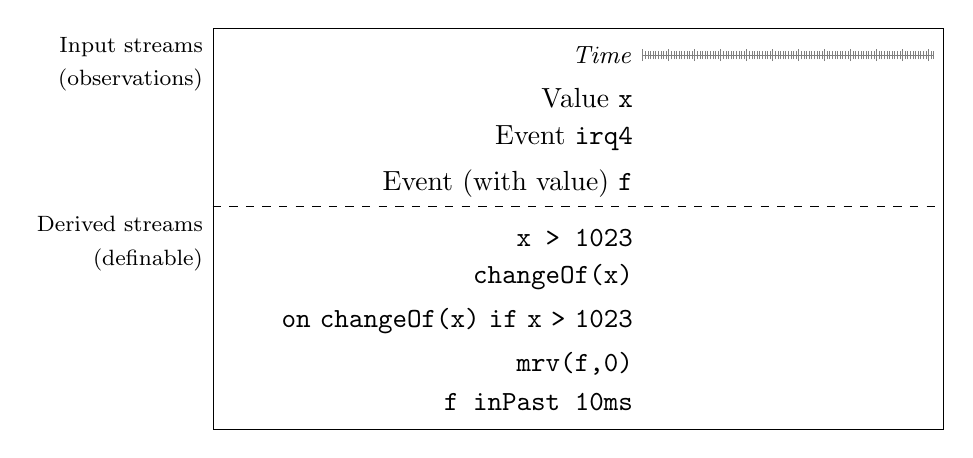
\begin{tikzpicture}

\matrix[column sep = 0.5em, draw] (m) {
  \node[anchor = east] {\small \textit{\textrm{Time}}}; \& \draw[help lines] (0,-0.05) grid[xstep=0.033] (3.7,0.05);
     \draw[gray] (0,-0.075) grid[xstep=0.33] (3.7,0.075); \\[0.5ex]
  \node[anchor = east] (m-1-2) {Value \texttt{x}}; \& \timing[name=m-2-2] at (0,-0.15) {2D{998}N(x1)2D{42}3D{2012}3D{1280}DD{10}DD{1404}};\\
%
  \node[anchor = east] (m-1-3) {Event \texttt{irq4}};
    \& \timing[name=m-2-3] at (0,-0.15) {ZZZ \n{} Z \n{} ZZZZ \n{} ZZ \n{} ZZZ \n{} Z}; \\
%
  \node[anchor = east] (end-inputs) {Event (with value) \texttt{f}};
    \& \timing[name = end-inputs-2] at (0,-0.15) {Z \n{17} ZZZZZZZ \n{98} Z \n{0} ZZZZ \n{23} Z}; \\[0.5em]
%
     \node[anchor = east] (m-1-5) {\texttt{x > 1023}};
  \& \timing[name=m-2-5] at (0,-0.15) {4L 6H 2L 2H}; \\
%
     \node[anchor = east] (m-1-6) {\texttt{changeOf(x)}};
  \& \timing[name=m-2-6] at (0,-0.15) {2Z \n{} 2Z \n{} 3Z \n{} 3Z \n{} 2Z \n{} 2Z}; \\
%
     \node[anchor = east, text width = 14.5em, align = right] (m-1-7) {
          \texttt{\textbf{on} changeOf(x) \textbf{if} x > 1023}};
  \& \timing[name=m-2-7] at (0,-0.15) {4Z \n{} 3Z \n{} 3Z 2Z \n{} 2Z}; \\
%
     \node[anchor = east] (m-1-8) {\texttt{mrv(f,0)}};
  \& \timing[name=m-2-8] at (0,-0.15) {D{0} 7D{17} D{98} 4D{0} D{23}}; \\
%
     \node[anchor = east] (m-1-9) {\texttt{f inPast 10ms}};
  \& \timing[name=m-2-9] at (0,-0.15) {L 2H 5L 3H 2L H}; \\
%
 };

\path[draw, dashed] (m.west|-end-inputs.south) edge (m.east|-end-inputs.south);

\path (m.north west) node[anchor = north east, align = right]
{\footnotesize{Input streams} \\ \footnotesize{(observations)}};

\path (m.west|-end-inputs.south) node[anchor = north east, align = right] {
  \footnotesize{Derived streams} \\ \footnotesize{(definable)}};

\end{tikzpicture}

  \caption{Visualization of \gls{tessla} stream model, taken from~\cite{Decker2016}}
\label{fig:chap2:sec_tessla:streams}
\end{figure}

The syntax of \gls{tessla} is pretty small, but can be used to define complex functions and specifications:

\begin{align*}
  spec\ \text{::= } &\textttbf{define } name[\textttbf{:}\ stype]\ \textttbf{:= } texpr |\\
                    & \textttbf{out } texpr |
                    spec\ spec\\
  texpr\ \text{:= } & expr[\textttbf{:}\ type] \\
  expr\ \text{:= }  & name \mid literal \mid name\textttbf{(}texpr(\textttbf{, }texpr)^*\textttbf{)}\\
  type\ \text{:= } & btype \mid stype \\
  stype\ \text{:= } & \textttbf{Signal<}btype\textttbf{>} \mid \textttbf{Events<}btype\textttbf{>}
\end{align*}

One of the main contributions of \gls{tessla} is the syntax which mimics modern programming languages and diverges from more clasical approaches in \gls{rv} that use more formal specification languages.
This is an important step to enable people without a strong theoretical background to include \gls{rv} techniques in their workflow.
While \gls{rv} has a lot of mechanisms to express specifications they often lack the ability to be intuitively understood.

While there exist many specification languages like \gls{ltl}~\citep{Pnueli77}, \gls{rltl}~\citep{Leucker2007}, \gls{ctl}~\citep{Clarke82} and many others they are geared heavily toward scientific work and theoretic reasoning.
When introducing new concepts like realtime this trend keeps up and formalism like \gls{tltl} from~\cite{Raskin1997}, \gls{stl} from~\cite{Maler2004} and \gls{mtl} from~\cite{Koymans1990} provide theoretical foundations to reason about realtime properties but formulas using theese logics are even harder to understand than their non realtime counterparts.

One approach to make \gls{rv} more usage friendly is \gls{salt} presented in~\cite{Bauer2006} which acts as frontend language to the more formal specification languages and can be transpiled into them.
\Gls{salt} unifies many different mechanism, like specification patterns, nested scopes, exceptions, regular expressions and realtime.
\Cref{listing:salt_example} shows an example specification in \gls{salt} taken and adapted from~\cite{Dwyer1999} which specifies that on all three floors in a building, calling the elevator at floor \(\mathit{i}\) implies that it may pass at most two times at that floor without opening its doors, and that it must finally open its doors at that floor within 60 seconds.

\begin{lstlisting}[float,breaklines=true,label=listing:salt_example,caption={[Example \gls{salt} specification with realtime operators]An example specification in the \gls{salt} language taken from \cite{Bauer2006} defining behaviour of an elevator.}]
define max_twice_at_floor_before_open(i) := always (occurring[<=2] atfloor_$i$ between inclusive optional call_$i$ , exclusive optional open_$i$)
define max_60s_before_open(i) := always (call_$i$ implies eventually timed[<=60.0] open_$i$)
assert allof enumerate[1..3] as floor in max_twice_at_floor_before_open(floor) and max_60s_before_open(floor)
\end{lstlisting}

This specification shows, how \gls{salt} specifications are more intuitively understandable thatn logic formulas, for example by allowing to split the formula in multiple parts and assign meaningful identifiers to subformulas.

\Gls{tessla} and the implemented runtime aims to combine many of the aspects that were presented in this Chapter: An understandable specification language like \gls{salt} that is able to express realtime properties, using streams of data as a central element like \gls{lola}, incorporate techniques from \gls{cep} like BeepBeep, and distribute the montitoring to many processors using Erlang and the actor model as used in \cite{Attard2016}.

\section{Trace Data}
\label{sec:related:traces}

Problem: Many traces don't carry timestamp (see DeCapo, CRV 15)
% \label{sec:related:drivertrace}
% DTrace PID

\url{http://lttng.org}
\url{http://diamon.org/ctf/}
\url{https://github.com/efficios/barectf}
\subsection{Debie}
\subsection{TraceBench}
\subsection{Aspect oriented programming}
\subsection{CIL}
\subsection{Google XRay}
\subsection{Sampling}
\subsection{LLVM}
\label{sec:related:traces:llvm}

